% 2.2
\section{Den aggregatorienterte datamodellen}

Så har vi den aggregatorienterte modellen, en metamodell som tillater den enkelte systemarkitekt å selv definere kompleksiteten til strukturen til sine egne dataenheter, slik at persisterte data er tilpasset applikasjonens struktur på sine dataobjekter i stedet for å tvinge vedkommende til å konformere med en forhåndsbestemt minste enhet, slik tilfellet er i den relasjonelle modellen. Denne fleksibiliteten i struktureringen av data er et sentralt fellestrekk nøkkelverdilagre som Dynamo og Redis deler med kolonnefamilie-lagre som Cassandra og HBase og dokumentdatabaser som MongoDB og CouchDB. Derfor definerer \cite{sadalage2013} en felles kategori for disse tre NoSQL-typene: ''Aggregatorienterte databasesystem''.

Begrepet ''aggregat'' (må ikke forveksles med det matematiske verbet som betegner en operasjon på en gruppe av tupler) er lånt fra domenedrevet design og er i kontekst av databasemodellering definert som en samling sammenknyttede objekter som en datamodellør ønsker å behandle som en enhet for datamanipulasjon og konsistenshandtering. Når komplekse aggregater aksesseres, gjøres det med et oppslag på én enkelt nøkkel, så får man både dataobjektet med den tilhørende nøkkelen samt eventuelle assosierte dataobjekter. Å utføre en tilsvarende lesing av to assosierte relasjoner i for eksempel MySQL krever først oppslag i en tabell på dens nøkkelverdi, deretter enda et oppslag på en fremmednøkkel i den assosierte tabellen, altså må en JOIN-operasjon utføres.

En aggregatmodell avgrenser den objektsrukturen til applikasjonens data som skal alltid skal omskrives i ett sett, hvilket betyr at når data i et nøstet objekt endres, blir hele aggregatobjektet i seg selv omskrevet. Aggregatet utgjør dermed en naturlig enhet for replikering i et distribuert databasesystem da hele den aggregerte objektstrukturen programvarens forretningslogikk jobber innenfor replikeres i sin helhet. En tuppel i en normalisert relasjon inneholder nødvendigvis ikke hele omfanget av dataobjektstrukturen forretningslogikken arbeider på, iallfall ikke uten en eller to JOIN-operasjon.

Aggregatobjektet er også en naturlig enhet for partisjonering: En stor mengde av individuelle aggregater er fra programvaresystemet sitt sitt standpunkt aksessert fullstendig uavhengig av hverandre, derfor kan de lemfeldig fordeles og kopieres utover et sett med uavhengig opererende databasenoder uten at objektenes plassering får konsekvenser for applikasjonens aksessmønster - skal en klient ha tak i ett spesifikt objekt kan den i prinsippet kontaktet én spesifikk databasenode i nettverket som er kjent for å holde på dette ønskede objektet. Å partisjonere tabeller i et relasjoner distribuert databasesystem kan, avhengig av de rådende assoiasjoner og fremmednøkkelbegrensninger, påvirke ytelsen til forskjellige spørringer etter forskjellige tupler som tilhører samme tabell, på grunn av algoritmen den distribuerte JOIN-operasjonen er implemntert med så vel som plasseringen av tupler med matchende assosiasjonsvariable (lik verdi for fremmednøkkel og primærnøkkel).

Lesing av aggregerte dataobjekter medfører at man med ett enkelt oppslag på én enkel nøkkel får både i pose og sekk. Aggregatmodellen er også en enklere datamodell å forholde seg til for de som programmerer selve applikasjonen som behandler dataene, av den enkle grunn at de slipper å skrive kode for å konvertere en lemfeldig liste av flate tupler. De enkelte aggregater, det vil si applikasjonsprogrammererens definisjon for databehandlingsenhet utgjør en naturlig enhet for replikering i en klynge av enkeltstående databasenoder. I et distribuert databasesystem gjelder det å minimalisere antall noder som kontaktes for hver spørring. Når konsepter settes sammen eksplisitt i datamodellen slik som vi ser i de fleksible dokumentstrukturene til Mongo, vet databasen hvilke dataenheter som skal aksesseres samtidig, og som derfor naturlig nok bør plasseres på én og samme node.

\cite{sadalage2013} kaller relasjonelle databaser og grafdatabaser for \textbf{aggregat-uvitende}. Deres datamodeller betrakter ikke aggregater eller sammensatte datastrukturer i deres dataoperasjoner. Aggregat-uvitenhet er ikke nødvendigvis et dårlig designvalg, ettersom det ikke alltid er opplagt for den enkelte webapplikasjonsutvikler hvilke enhetsbegrensinger i datamodellen som er logiske, iallfall ikke før datamodellen er definert for første gang og revidert to til tre ganger i løpet av utviklingsprosessen. Den lagrede dataen kan ha mange forskjellige brukskontekster, avhengig av applikasjonens funksjonelle krav som ofte blir forandret underveis i applikasjonens livssyklus.

En enkelt aggregatstruktur kan ikke medføre optimale spørringsytelse for alle mulige brukskontekster. Her gjelder det for utvikleren å prioritere den mest typiske leseoperasjonen tjenesten utsettes for. Hvis applikasjonen ikke har en slik primær aksess – struktur på dataobjektene kan man like godt modellere dem på et aggregat-uvitende vis. I en aggregat-uvitende modell har brukskonteksten ingen innvirkning på spørringen, fordi operasjonsenheten er én enkelt tuppel i MariaDB uansett hvordan konseptene er satt sammen.

Aggregatorienterte databasesystemer innehar ikke ACID - egenskapene som vi finner hos transaksjoner i relasjonelle databasesystemer. Imidlertid støtter de naturlig atomiske manipulasjoner på ett eneste aggregat av gangen. Ved nøkkeloppslag får man hele dataobjektet den tilkoplete applikasjonen leser og manipulerer, Samtidighetskontroll ved operasjoner på flere aggregater må følgelig handteres i kildekoden til applikasjonen, spørring for spørring, der et unntak må kastes hvis én av spørringene mislykkes. Å emulere transaksjoner i enkeltaggregater inngår som en viktig faktor i hvordan aggregatene defineres i datamodellen \citep{sadalage2013}.

% 2.2.1
\subsection{Design av aggregatmodeller}

% DDI: Denormalisering, duplisering og intelligentte fremmednøkler

% Legg inn eksempel av aggregatmodell konvertert fra figur 1
Slik kan en generisk aggregatmodell, uttrykt i UML, ekvivalent til datamodellen fra \ref{fig1} se ut.

% Figur 2
\begin{figure}[ht]
    \centering
    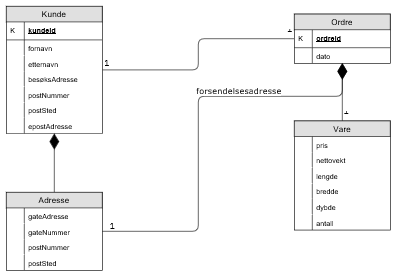
\includegraphics{fig/NettbutikkAggregatModell.png}
    \caption{Aggregatdiagram med to forskjellige entiter for den samme tjenesten fra \ref{fig1}.}
    \label{fig2}
\end{figure}

Denne figuren  presenterer to forskjellige aggregater, \texttt{Kunde} og \texttt{Ordre}. Forbindelsen mellom disse to denoterer 
Ved modellering av aggregater må man avveie mellom hvor stort hvert enkelt aggregatobjekt i en applikasjon kan bli og hvor mange forskjellige aggregatentiter applikasjonen kan ha. Med to nivaåer av nøstede lister av objekter innen ett aggregat kan besvarelse av ett enkelt oppslag på én spesifikk nøkkel 

% Skriv om tre ulike aggregat - orienterte datamodeller - Segway til påfølgende delkapitler
Fowler og Sadalage omtaler tre unike datamodeller som opererer med aggregater. Nøkkelverdimodellen behandler det enkelte aggregat som en ugjennomsiktig helhet \citep{sadalage2013}. Altså går det ikke an å hente deler av aggregatet ved et nøkkeloppslag. Dokumentmodellen eksponerer aggregatet til databasen, og tillater dermed delvise spørringer. I og med at dokumentmodellen også er skjemaløs går det ikke an å optimalisere spørringer på hele eller deler av aggregatet. Kolonnefamilier inndeler aggregatet i grupper, noe som tillater databasen å operere på hver av disse gruppene som en egen dataenhet, lik som attributter i tuplene i den relasjonelle modellen. Selv om kolonnefamilier til dels ofrer den komplette skjemaløsheten som vi ser i nøkkelverdimodellen, har databasen nå mulighet til å nytte eksponeringen av attributter/kolonner til å optimalisere aksesseringer og oppdatere separate kolonner.

% 2.2.2
\subsection{Nøkkel-verdi-modellen}

Nøkkelverdilagre er den type NoSQL-DBMS med den enkleste datamodell. Spørringer inndeles hovedsaklig i tre kategorier: GET, PUT og DELETE. 
